\documentclass{article}
\usepackage[a4paper]{geometry}
\usepackage{amsmath}
\usepackage{amsfonts}
\usepackage{amssymb}
\usepackage{graphicx}
\usepackage{subcaption}
\usepackage{float}
\graphicspath{{./images/}}
\begin{document}
\begin{center}
	{\LARGE Exercise 6}\linebreak
	{\large [Avik Banerjee (3374885), Soumyadeep Bhattacharjee (3375428)]}
\end{center}
\textit{Text in italics are notes taken during the exercise}
\section{Planning and Learning}
\begin{enumerate}
	\item[a)]Considering a large enough n and overlooking the additional computation cost and memory requirements for n-step bootstrapping methods, Dyna would still perform better. In n-step bootstrapping, the update is delayed and since the states are updated sequentially, it requires time to transfer the updated information.
	
	In the Dyna method, learning and planning are accomplished by the same algorithm, operating on real experience for learning and on simulated experience for planning, thus quickly synthesizing into an optimal trajectory. 
	\item[b)] Both DynaQ and DynaQ+ can handle a situation where the environment gets worse, and can successfully find the optimal policy
	However, a problem is caused by an improvement of environment in the maze. After 3000 steps, a shorter path is revealed along the right side, without changing the longer path (upper right). 
	
	The model of the DynaQ agent did not figure out the shortcut, so the more it planned, the less likely it was to explore to the right and discover the path, even with an $\epsilon$-greedy policy. It may find a trajectory that works (but is suboptimal) and then spend a long time to take enough exploratory analysis to discover an optimal policy.
	
	The Dyna-Q+ agent solved the shortcut maze as it is encouraged to find changes in the environment due to increased exploration. It keeps track of how many time steps have elapsed for each state–action pair since the pair was last tried in a real interaction with the environment. The more time that has elapsed, there is presumably a greater chance that the dynamics of this pair has changed and that the model of it is incorrect. To encourage behavior that tests long-untried actions, a special “bonus reward” is given on simulated experiences involving these actions. This encourages the agent to keep testing all accessible state transitions and to find long sequences of actions to carry out such tests.
\end{enumerate}
\section{n-step sarsa on the FrozenLake}
\begin{figure}[H]
	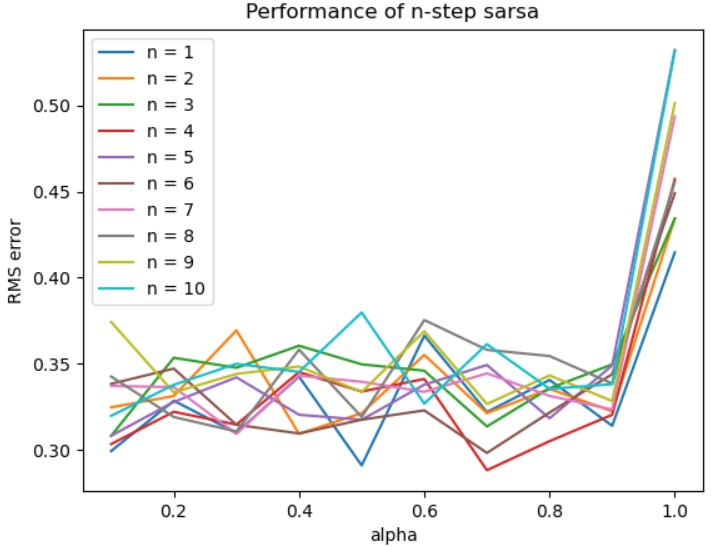
\includegraphics[width=0.5\linewidth]{graph.jpg}
\end{figure}
\end{document}